% Simplified main-text Figure 2: single-panel mediator DAG (TikZ standalone).
%
% Built in TikZ (compiled with local MacTeX, not the renv/ggplot stack) because
% DAGs are TikZ's home turf and the renv library on Dropbox CloudStorage makes R
% plotting pathologically slow here. Style + palette adopt the agentic-ai-tool-
% chain "Data-science workflow" figure: Inter sans, and the stage fills
% (sage green, periwinkle blue, dusty red, grey).
%
% Layout: the five control (MSAS) boxes sit on one row inside a dashed dusty-red
% plate (centred label, with headroom above the boxes). No bold; node text 8pt.
% No in-figure legend (the manuscript caption carries the colour key).
%
% Build (fontspec + Inter -> xelatex; run twice for the fit plate):
%   xelatex mediator-simplified.tex
% In a sandboxed shell the TeX font cache must be writeable, e.g.
%   TEXMFVAR=$TMPDIR/texmf-var TEXMFCACHE=$TMPDIR/texmf-cache xelatex ...
% (lualatex is interchangeable but needs the same cache redirect.)
% Output: mediator-simplified.pdf  ->  outputs/figures/final/fig-2-dag-mediator-simplified.pdf

\documentclass[border=8pt]{standalone}
\usepackage{fontspec}
\setsansfont{Inter}
\renewcommand{\familydefault}{\sfdefault}
\usepackage{tikz}
\usetikzlibrary{arrows.meta, positioning, fit, backgrounds, calc}

% palette — fills from the Data-science workflow figure
\definecolor{stageSetup}{HTML}{CFD8EA}   % periwinkle blue -> outcome
\definecolor{stageLang}{HTML}{CFDFCD}    % sage green      -> exposure
\definecolor{stageAuth}{HTML}{E3C2BC}    % dusty red       -> adjustment set
\definecolor{stageOut}{HTML}{D9D9D9}     % grey            -> mediator
\definecolor{dark}{HTML}{1E293B}
\definecolor{slate}{HTML}{64748B}
\definecolor{linegreen}{HTML}{3F7E4E}    % causal edge (darker sage)
\definecolor{linered}{HTML}{A85D52}      % adjustment-set border / back-door edges (darker dusty red)

\begin{document}
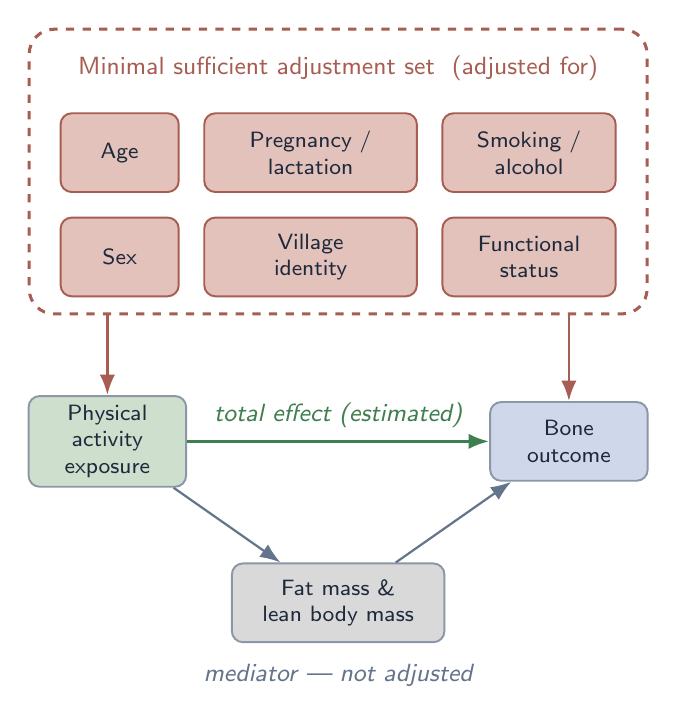
\begin{tikzpicture}[
  font=\sffamily\footnotesize,                 % Inter, 8pt node text, no bold
  exposure/.style={rectangle, rounded corners=4pt, draw=slate!75, line width=0.7pt,
                   fill=stageLang, text=dark, align=center,
                   minimum width=2cm, minimum height=1cm},
  outcome/.style={rectangle, rounded corners=4pt, draw=slate!75, line width=0.7pt,
                  fill=stageSetup, text=dark, align=center,
                  minimum width=2cm, minimum height=1cm},
  mediator/.style={rectangle, rounded corners=4pt, draw=slate!75, line width=0.7pt,
                   fill=stageOut, text=dark, align=center,
                   minimum width=2.7cm, minimum height=1cm},
  msas/.style={rectangle, rounded corners=4pt, draw=linered, line width=0.7pt,
               fill=stageAuth, text=dark, align=center,
               minimum width=1.5cm, minimum height=1.0cm},
  causal/.style={-{Latex[length=2.6mm]}, draw=linegreen, line width=1.2pt},
  backdoor/.style={-{Latex[length=2.6mm]}, draw=linered, line width=1.0pt},
  mediated/.style={-{Latex[length=2.6mm]}, draw=slate, line width=0.8pt},
  anno/.style={font=\sffamily\itshape\small}
]

  % --- minimal sufficient adjustment set: 2 rows x 3 cols (village IS part of the set) ---
  % top row:    age | pregnancy/lactation | smoking/alcohol  (per-column widths)
  \node[msas] (age) at (0, 2.95)         {Age};
  \node[msas, minimum width=2.7cm, right=0.3cm of age] (pl)   {Pregnancy /\\ lactation};
  \node[msas, minimum width=2.2cm, right=0.3cm of pl]  (smk)  {Smoking /\\ alcohol};
  % bottom row: sex | village identity     | functional status (aligned under top row)
  \node[msas, below=0.3cm of age] (sex)  {Sex};
  \node[msas, minimum width=2.7cm, below=0.3cm of pl]  (vill) {Village\\ identity};
  \node[msas, minimum width=2.2cm, below=0.3cm of smk] (fs)   {Functional\\ status};

  % centred label above the top row (included in the plate fit -> tight top)
  \node[anchor=south, font=\sffamily\small, text=linered] (setlabel)
    at ($(age.north west)!0.5!(smk.north east) + (0, 0.28)$)
    {Minimal sufficient adjustment set\ \ (adjusted for)};

  % --- dashed dusty-red adjustment-set plate (tight fit around label + all six boxes) ---
  \begin{scope}[on background layer]
    \node[draw=linered, line width=1.1pt, dashed, rounded corners=9pt,
          fit=(setlabel)(age)(pl)(smk)(sex)(vill)(fs),
          inner xsep=11pt, inner ysep=6pt] (plate) {};
  \end{scope}

  % --- exposure / outcome / mediator: span the FULL width of the adjustment-set plate ---
  % Anchored west/east at a COMMON y, so both nodes are vertically centred on the (horizontal)
  % exposure->outcome edge regardless of their differing heights (the exposure node is taller);
  % span = dashed-box width, so the causal arrow carries the "total effect (estimated)" label.
  \node[exposure, anchor=west] (pa)   at ([yshift=-1.6cm]plate.south west) {Physical\\ activity\\ exposure};
  \node[outcome,  anchor=east] (bone) at ([yshift=-1.6cm]plate.south east) {Bone\\ outcome};
  \node[mediator] (bc) at ($(pa)!0.5!(bone)-(0,2.05)$) {Fat mass \&\\ lean body mass};

  % --- edges ---
  \draw[causal] (pa) -- node[anno, above, text=linegreen, yshift=1pt]
        {total effect (estimated)} (bone);
  \draw[mediated] (pa) -- (bc);
  \draw[mediated] (bc) -- (bone);
  \draw[backdoor] (plate.south -| pa) -- (pa);
  \draw[backdoor] (plate.south -| bone) -- (bone);

  % mediator annotation
  \node[anno, text=slate, below=4pt of bc] {mediator --- not adjusted};

\end{tikzpicture}
\end{document}
